% Document template for ANS Journals
%DIF LATEXDIFF DIFFERENCE FILE
%DIF DEL main.tex       Fri Dec  1 17:11:44 2023
%DIF ADD revision.tex   Wed Jan 31 19:25:45 2024
% Options: footnoteAtEnd - Places all footnotes at the end of document
%               Usage: \documentclass[footnoteAtEnd]{style/nseJournal}
\documentclass{style/nseJournal}

\usepackage[acronym,toc]{glossaries}
%DIF 7c7
%DIF < \newacronym{ANL}{ANL}{Argonne National Laboratory}
\newacronym{ANN}{ANN}{Artificial Neural Network}
\newacronym{API}{API}{Application Programming Interface}
\newacronym{ATR}{ATR}{Advanced Test Reactor}
\newacronym{B4C}{B4C}{boron carbide}
\newacronym{BC}{BC}{boundary condition}
\newacronym{BNCT}{BNCT}{Boron Neutron Capture Therapy}
\newacronym{BOC}{BOC}{beginning of the equilibrium cycle}
\newacronym{BSD}{BSD}{Berkeley Software Distribution}
\newacronym{BWR}{BWR}{Boiling Water Reactor}
\newacronym{CAISO}{CAISO}{California ISO}
\newacronym{CAPP}{CAPP}{Core Analyzer for Pebble and Prism type VHTRs}
\newacronym{CEA}{CEA}{Commissariat a l'Energie Atomique}
\newacronym{CFD}{CFD}{computational fluid dynamics}
\newacronym{CO2}{CO$_2$}{carbon dioxide}
\newacronym{CNN}{CNN}{Convolutional Neural Network}
\newacronym{CR}{CR}{control rod}
\newacronym{CRAM}{CRAM}{Chebyshev Rational Approximation Method}
\newacronym{CRP}{CRP}{Coordinated Research Project}
\newacronym{CZP}{CZP}{Cold Zero Power}
\newacronym{DCC}{DCC}{depressurized conduction cool-down}
\newacronym{DOE}{DOE}{Department of Energy}
\newacronym[\glslongpluralkey={degrees of freedom}]{DoF}{DoF}{degree of freedom}
\newacronym{DT}{DT}{Decision Tree}
\newacronym{DTR}{DTR}{Decision Tree Regression}
\newacronym{EOC}{EOC}{end of the equilibrium cycle}
\newacronym{FCEV}{FCEV}{Fuel Cell Electric Vehicle}
\newacronym{FDM}{FDM}{Finite Difference Method}
\newacronym{FEM}{FEM}{Finite Element Method}
\newacronym{FNN}{FNN}{Feedforward Neural Network}
\newacronym{FVM}{FVM}{Finite Volume Method}
\newacronym[\glslongpluralkey={greenhouse gases}]{GHG}{GHG}{greenhouse gas}
\newacronym[\glslongpluralkey={Gaussian processes}]{GP}{GP}{Gaussian process}
\newacronym{GRS}{GRS}{Gesellschaft für Anlagen und Reaktorsicherheit}
\newacronym{GT-MHR}{GT-MHR}{Gas Turbine-Modular Helium Reactor}
\newacronym{H2}{H$_2$}{hydrogen}
\newacronym{He}{He}{helium}
\newacronym{HFIR}{HFIR}{High Flux Isotope Reactor}
\newacronym{HFP}{HFP}{Hot Full Power}
\newacronym{HPC}{HPC}{high-performane computing}
\newacronym{HPCC}{HPCC}{high-pressure conduction cool-down}
\newacronym{HTE}{HTE}{High-Temperature Electrolysis}
\newacronym{HTGR}{HTGR}{High-Temperature Gas-Cooled Reactor}
\newacronym{HTR}{HTR}{High Temperature Reactor}
\newacronym{HTTR}{HTTR}{High-Temperature engineering Test Reactor}
\newacronym{HZDR}{HZDR}{Helmholtz-Zentrum Dresden-Rossendorf}
\newacronym{IAEA}{IAEA}{International Atomic Energy Agency}
\newacronym{icap}{iCAP}{Illinois Climate Action Plan}
\newacronym{INL}{INL}{Idaho National Laboratory}
\newacronym{IPyC}{IPyC}{inner pyrolytic carbon}
\newacronym{JFNK}{JFNK}{Jacobian-Free Newton-Krylov}
\newacronym{KAERI}{KAERI}{Korea Atomic Energy Research Institute}
\newacronym{Keff}{k$_{eff}$}{multiplication factor}
\newacronym{KNN}{KNN}{K-Nearest Neighbors}
\newacronym{LANL}{LANL}{Los Alamos National Laboratory}
\newacronym{LBP}{LBP}{Lumped Burnable Poison}
\newacronym{LEU}{LEU}{low-enriched uranium}
\newacronym{HEU}{HEU}{highly-enriched uranium}
\newacronym{LGPL}{LGPL}{Lesser GNU Public License}
\newacronym{LOCA}{LOCA}{loss-of-coolant accident}
\newacronym{LOFW}{LOFW}{loss-of-feedwater}
\newacronym{LOFA}{LOFA}{loss-of-flow accident}
\newacronym{LogR}{LogR}{Logistic Regression}
\newacronym{LPCC}{LPCC}{low-pressure conduction cool-down}
\newacronym{LR}{LR}{Linear Regression}
\newacronym{LSTM}{LSTM}{Long Short-Term Memory Network}
\newacronym{LTE}{LTE}{Low-Temperature Electrolysis}
\newacronym{LWR}{LWR}{Light Water Reactor}
\newacronym{MOAA}{MOAA}{MCNP-ORIGEN Activation Automation}
\newacronym{MC}{MC}{Monte Carlo}
\newacronym{MHTGR}{MHTGR}{Modular High-Temperature Gas-Cooled Reactor}
\newacronym{ML}{ML}{machine learning}
\newacronym{MMR}{MMR}{Micro Modular Reactor}
\newacronym{MOC}{MOC}{middle of the equilibrium cycle}
\newacronym{MOX}{MOX}{Mixed-Oxide}
\newacronym{MOOSE}{MOOSE}{Multi-physics Object-Oriented Simulation Environment}
\newacronym{MPI}{MPI}{Message Passing Interface}
\newacronym{MAE}{MAE}{Mean Absolute Error}
\newacronym{MSE}{MSE}{Mean Squared Error}
\newacronym{MSR}{MSR}{Molten Salt Reactor}
\newacronym{MTR}{MTR}{material-testing reactor}
\newacronym{ND}{ND}{net demand}
\newacronym{NEA}{NEA}{Nuclear Energy Agency}
\newacronym{NEM}{NEM}{Nodal Expansion Method}
\newacronym{NGNP}{NGNP}{Next Generation Nuclear Power}
\newacronym{NPP}{NPP}{Nuclear Power Plant}
\newacronym{NRC}{NRC}{Nuclear Regulatory Commission}
\newacronym{NSC}{NSC}{Nuclear Science Committee}
\newacronym{OECD}{OECD}{Organisation for Economic Co-operation and Development}
\newacronym{OPyC}{OPyC}{outer pyrolytic carbon}
\newacronym{ORNL}{ORNL}{Oak Ridge National Laboratory}
\newacronym{OS}{OS}{Operator-Splitting}
\newacronym{PBMR}{PBMR}{Pebble Bed Modular Reactor}
\newacronym{PDE}{PDE}{Partial Differential Equation}
\newacronym{PIE}{PIE}{post-irradiation examination}
\newacronym{PMR}{PMR}{Prismatic Modular Reactor}
\newacronym{PV}{PV}{photovoltaics}
\newacronym{PWR}{PWR}{Pressurized Water Reactor}
\newacronym{RF}{RF}{Random Forest}
\newacronym{RFR}{RFR}{Random Forest Regression}
\newacronym{RNN}{RNN}{Recurrent Neural Network}
\newacronym{RPV}{RPV}{Reactor Pressure Vessel}
\newacronym{RSC}{RSC}{Reserve Shutdown Control}
\newacronym{RSD}{RSD}{Relative Standard Deviation}
\newacronym{R2S}{R2S}{Rigorous 2-Step}
\newacronym{SD}{SD}{Standard Deviation}
\newacronym{SI}{SI}{Sulfur-Iodine}
\newacronym{SiC}{SiC}{silicon carbide}
\newacronym{SMR}{SMR}{Small Modular Reactor}
\newacronym{SNU}{SNU}{Seoul National University}
\newacronym{SOEC}{SOEC}{Solid Oxide Electrolysis Cells}
\newacronym{SP3}{SP$_3$}{Simplified P$_3$}
\newacronym{SVM}{SVM}{Support Vector Machine}
\newacronym{SVR}{SVR}{Support Vector Regression}
\newacronym{TFHR}{TFHR}{Fluoride-salt-cooled High-temperature Reactor}
\newacronym{TIP}{TIP}{transverse integration procedure}
\newacronym{TRISO}{TRISO}{Tristructural Isotropic}
\newacronym{TREAT}{TREAT}{Transient Reactor Test Facility}
\newacronym{UIUC}{UIUC}{University of Illinois at Urbana-Champaign}
\newacronym{UIF}{UIF}{user input file}
\newacronym{UNIST}{UNIST}{Ulsan National Institute of Science and Technology}
\newacronym{UK}{UK}{United Kingdom}
\newacronym{UMICH}{UMICH}{University of Michigan}
\newacronym{UQ}{UQ}{Uncertainty Quantification}
\newacronym{US}{US}{United States}
\newacronym{USNC}{USNC}{Ultra Safe Nuclear Corporation}
\newacronym{VHTR}{VHTR}{Very High-Temperature Gas-Cooled Reactor}
\newacronym{WRM}{WRM}{weighted residual method}
%\newacronym{<++>}{<++>}{<++>}
%\newacronym{<++>}{<++>}{<++>}

%DIF -------
\newacronym{ANL}{ANL}{Argonne National Laboratory}
\newacronym{ANN}{ANN}{Artificial Neural Network}
\newacronym{API}{API}{Application Programming Interface}
\newacronym{ATR}{ATR}{Advanced Test Reactor}
\newacronym{B4C}{B4C}{boron carbide}
\newacronym{BC}{BC}{boundary condition}
\newacronym{BNCT}{BNCT}{boron neutron capture therapy}
\newacronym{BOC}{BOC}{beginning of the equilibrium cycle}
\newacronym{BSD}{BSD}{Berkeley Software Distribution}
\newacronym{BWR}{BWR}{Boiling Water Reactor}
\newacronym{CAISO}{CAISO}{California ISO}
\newacronym{CAPP}{CAPP}{Core Analyzer for Pebble and Prism type VHTRs}
\newacronym{CEA}{CEA}{Commissariat a l'Energie Atomique}
\newacronym{CFD}{CFD}{computational fluid dynamics}
\newacronym{CO2}{CO$_2$}{carbon dioxide}
\newacronym{CNN}{CNN}{Convolutional Neural Network}
\newacronym{CR}{CR}{control rod}
\newacronym{CRAM}{CRAM}{Chebyshev Rational Approximation Method}
\newacronym{CRP}{CRP}{Coordinated Research Project}
\newacronym{CZP}{CZP}{Cold Zero Power}
\newacronym{DCC}{DCC}{depressurized conduction cool-down}
\newacronym{DOE}{DOE}{Department of Energy}
\newacronym[\glslongpluralkey={degrees of freedom}]{DoF}{DoF}{degree of freedom}
\newacronym{DT}{DT}{Decision Tree}
\newacronym{DTR}{DTR}{Decision Tree Regression}
\newacronym{EOC}{EOC}{end of the equilibrium cycle}
\newacronym{FCEV}{FCEV}{Fuel Cell Electric Vehicle}
\newacronym{FDM}{FDM}{Finite Difference Method}
\newacronym{FEM}{FEM}{Finite Element Method}
\newacronym{FNN}{FNN}{Feedforward Neural Network}
\newacronym{FVM}{FVM}{Finite Volume Method}
\newacronym[\glslongpluralkey={greenhouse gases}]{GHG}{GHG}{greenhouse gas}
\newacronym[\glslongpluralkey={Gaussian processes}]{GP}{GP}{Gaussian process}
\newacronym{GRS}{GRS}{Gesellschaft für Anlagen und Reaktorsicherheit}
\newacronym{GT-MHR}{GT-MHR}{Gas Turbine-Modular Helium Reactor}
\newacronym{H2}{H$_2$}{hydrogen}
\newacronym{He}{He}{helium}
\newacronym{HFIR}{HFIR}{High Flux Isotope Reactor}
\newacronym{HFP}{HFP}{Hot Full Power}
\newacronym{HPC}{HPC}{high-performane computing}
\newacronym{HPCC}{HPCC}{high-pressure conduction cool-down}
\newacronym{HTE}{HTE}{High-Temperature Electrolysis}
\newacronym{HTGR}{HTGR}{high-temperature gas-cooled reactor}
\newacronym{HTR}{HTR}{High Temperature Reactor}
\newacronym{HTTR}{HTTR}{High-Temperature engineering Test Reactor}
\newacronym{HZDR}{HZDR}{Helmholtz-Zentrum Dresden-Rossendorf}
\newacronym{IAEA}{IAEA}{International Atomic Energy Agency}
\newacronym{icap}{iCAP}{Illinois Climate Action Plan}
\newacronym{INL}{INL}{Idaho National Laboratory}
\newacronym{IPyC}{IPyC}{inner pyrolytic carbon}
\newacronym{JFNK}{JFNK}{Jacobian-Free Newton-Krylov}
\newacronym{KAERI}{KAERI}{Korea Atomic Energy Research Institute}
\newacronym{Keff}{k$_{eff}$}{multiplication factor}
\newacronym{KNN}{KNN}{K-Nearest Neighbors}
\newacronym{LANL}{LANL}{Los Alamos National Laboratory}
\newacronym{LBP}{LBP}{Lumped Burnable Poison}
\newacronym{LEU}{LEU}{low-enriched uranium}
\newacronym{HEU}{HEU}{highly-enriched uranium}
\newacronym{LGPL}{LGPL}{Lesser GNU Public License}
\newacronym{LOCA}{LOCA}{loss-of-coolant accident}
\newacronym{LOFW}{LOFW}{loss-of-feedwater}
\newacronym{LOFA}{LOFA}{loss-of-flow accident}
\newacronym{LogR}{LogR}{Logistic Regression}
\newacronym{LPCC}{LPCC}{low-pressure conduction cool-down}
\newacronym{LR}{LR}{Linear Regression}
\newacronym{LSTM}{LSTM}{Long Short-Term Memory Network}
\newacronym{LTE}{LTE}{Low-Temperature Electrolysis}
\newacronym{LWR}{LWR}{Light Water Reactor}
\newacronym{MOAA}{MOAA}{MCNP-ORIGEN Activation Automation}
\newacronym{MC}{MC}{Monte Carlo}
\newacronym{MHTGR}{MHTGR}{Modular High-Temperature Gas-Cooled Reactor}
\newacronym{ML}{ML}{machine learning}
\newacronym{MMR}{MMR}{Micro Modular Reactor}
\newacronym{MOC}{MOC}{middle of the equilibrium cycle}
\newacronym{MOX}{MOX}{Mixed-Oxide}
\newacronym{MOOSE}{MOOSE}{Multi-physics Object-Oriented Simulation Environment}
\newacronym{MPI}{MPI}{Message Passing Interface}
\newacronym{MAE}{MAE}{Mean Absolute Error}
\newacronym{MSE}{MSE}{Mean Squared Error}
\newacronym{MSR}{MSR}{Molten Salt Reactor}
\newacronym{MTR}{MTR}{material-testing reactor}
\newacronym{ND}{ND}{net demand}
\newacronym{NEA}{NEA}{Nuclear Energy Agency}
\newacronym{NEM}{NEM}{Nodal Expansion Method}
\newacronym{NGNP}{NGNP}{Next Generation Nuclear Power}
\newacronym{NPP}{NPP}{Nuclear Power Plant}
\newacronym{NRC}{NRC}{Nuclear Regulatory Commission}
\newacronym{NSC}{NSC}{Nuclear Science Committee}
\newacronym{OECD}{OECD}{Organisation for Economic Co-operation and Development}
\newacronym{OPyC}{OPyC}{outer pyrolytic carbon}
\newacronym{ORNL}{ORNL}{Oak Ridge National Laboratory}
\newacronym{OS}{OS}{Operator-Splitting}
\newacronym{PBMR}{PBMR}{Pebble Bed Modular Reactor}
\newacronym{PDE}{PDE}{Partial Differential Equation}
\newacronym{PIE}{PIE}{post-irradiation examination}
\newacronym{PMR}{PMR}{Prismatic Modular Reactor}
\newacronym{PV}{PV}{photovoltaics}
\newacronym{PWR}{PWR}{pressurized water reactor}
\newacronym{RF}{RF}{Random Forest}
\newacronym{RFR}{RFR}{Random Forest Regression}
\newacronym{RNN}{RNN}{Recurrent Neural Network}
\newacronym{RPV}{RPV}{Reactor Pressure Vessel}
\newacronym{RSC}{RSC}{Reserve Shutdown Control}
\newacronym{RSD}{RSD}{Relative Standard Deviation}
\newacronym{R2S}{R2S}{Rigorous 2-Step}
\newacronym{SD}{SD}{Standard Deviation}
\newacronym{SI}{SI}{Sulfur-Iodine}
\newacronym{SiC}{SiC}{silicon carbide}
\newacronym{SMR}{SMR}{Small Modular Reactor}
\newacronym{SNU}{SNU}{Seoul National University}
\newacronym{SOEC}{SOEC}{Solid Oxide Electrolysis Cells}
\newacronym{SP3}{SP$_3$}{Simplified P$_3$}
\newacronym{SVM}{SVM}{Support Vector Machine}
\newacronym{SVR}{SVR}{Support Vector Regression}
\newacronym{TFHR}{TFHR}{Fluoride-salt-cooled High-temperature Reactor}
\newacronym{TIP}{TIP}{transverse integration procedure}
\newacronym{TRISO}{TRISO}{Tristructural Isotropic}
\newacronym{TREAT}{TREAT}{Transient Reactor Test Facility}
\newacronym{UIUC}{UIUC}{University of Illinois at Urbana-Champaign}
\newacronym{UIF}{UIF}{user input file}
\newacronym{UNIST}{UNIST}{Ulsan National Institute of Science and Technology}
\newacronym{UK}{UK}{United Kingdom}
\newacronym{UMICH}{UMICH}{University of Michigan}
\newacronym{UQ}{UQ}{uncertainty quantification}
\newacronym{US}{US}{United States}
\newacronym{USNC}{USNC}{Ultra Safe Nuclear Corporation}
\newacronym{VHTR}{VHTR}{Very High-Temperature Gas-Cooled Reactor}
\newacronym{WRM}{WRM}{weighted residual method}
%\newacronym{<++>}{<++>}{<++>}
%\newacronym{<++>}{<++>}{<++>}
 %DIF > 
%DIF -------
\usepackage{booktabs}
\usepackage{relsize}
%DIF PREAMBLE EXTENSION ADDED BY LATEXDIFF
%DIF UNDERLINE PREAMBLE %DIF PREAMBLE
\RequirePackage[normalem]{ulem} %DIF PREAMBLE
\RequirePackage{color}\definecolor{RED}{rgb}{1,0,0}\definecolor{BLUE}{rgb}{0,0,1} %DIF PREAMBLE
\providecommand{\DIFadd}[1]{{\protect\color{blue}\uwave{#1}}} %DIF PREAMBLE
\providecommand{\DIFdel}[1]{{\protect\color{red}\sout{#1}}}                      %DIF PREAMBLE
%DIF SAFE PREAMBLE %DIF PREAMBLE
\providecommand{\DIFaddbegin}{} %DIF PREAMBLE
\providecommand{\DIFaddend}{} %DIF PREAMBLE
\providecommand{\DIFdelbegin}{} %DIF PREAMBLE
\providecommand{\DIFdelend}{} %DIF PREAMBLE
\providecommand{\DIFmodbegin}{} %DIF PREAMBLE
\providecommand{\DIFmodend}{} %DIF PREAMBLE
%DIF FLOATSAFE PREAMBLE %DIF PREAMBLE
\providecommand{\DIFaddFL}[1]{\DIFadd{#1}} %DIF PREAMBLE
\providecommand{\DIFdelFL}[1]{\DIFdel{#1}} %DIF PREAMBLE
\providecommand{\DIFaddbeginFL}{} %DIF PREAMBLE
\providecommand{\DIFaddendFL}{} %DIF PREAMBLE
\providecommand{\DIFdelbeginFL}{} %DIF PREAMBLE
\providecommand{\DIFdelendFL}{} %DIF PREAMBLE
%DIF LISTINGS PREAMBLE %DIF PREAMBLE
\RequirePackage{listings} %DIF PREAMBLE
\RequirePackage{color} %DIF PREAMBLE
\lstdefinelanguage{DIFcode}{ %DIF PREAMBLE
%DIF DIFCODE_UNDERLINE %DIF PREAMBLE
  moredelim=[il][\color{red}\sout]{\%DIF\ <\ }, %DIF PREAMBLE
  moredelim=[il][\color{blue}\uwave]{\%DIF\ >\ } %DIF PREAMBLE
} %DIF PREAMBLE
\lstdefinestyle{DIFverbatimstyle}{ %DIF PREAMBLE
	language=DIFcode, %DIF PREAMBLE
	basicstyle=\ttfamily, %DIF PREAMBLE
	columns=fullflexible, %DIF PREAMBLE
	keepspaces=true %DIF PREAMBLE
} %DIF PREAMBLE
\lstnewenvironment{DIFverbatim}{\lstset{style=DIFverbatimstyle}}{} %DIF PREAMBLE
\lstnewenvironment{DIFverbatim*}{\lstset{style=DIFverbatimstyle,showspaces=true}}{} %DIF PREAMBLE
%DIF END PREAMBLE EXTENSION ADDED BY LATEXDIFF

\begin{document}

\title{Delayed heating calculations using the MCNP-ORIGEN Activation Automation tool}

% Use the \addAuthor macro to add authors in the order they should appear. The second argument corresponds to
% the affiliation declared below.
% The corresponding author should be wrapped in \correspondingAuthor
\addAuthor{\correspondingAuthor{Roberto E. Fairhurst-Agosta}}{a}
% The corresponding author's email can be specified using \correspondingEmail
\correspondingEmail{ref3@illinois.edu}
\addAuthor{Tomasz Kozlowski}{a}

% Affiliations can be added in the order they should appear. For breaks in addresses, use either \\ or \tabularnewline
\addAffiliation{a}{Department of Nuclear, Plasma, and Radiological Engineering\\ University of Illinois Urbana-Champaign, Urbana, IL 61801}

% Add keywords to appear in Abstract in the order they should appear
\addKeyword{Delayed Heating}
\addKeyword{MCNP}
\addKeyword{ORIGEN}
\addKeyword{ATR}
\addKeyword{RA-6}


\titlePage

\begin{abstract}
An accurate assessment of the deposited energy across a reactor geometry allows a better determination of the heat removal requirements and ensure effective cooling after shutdown.
This work discusses several methods in detail that target the heat deposition in specific reactor regions, leading to a choice of a prevalent method for the calculation workflow.
This article introduces a delayed heating calculation workflow based on the formal 3-step process.
The workflow relies on the MCNP-ORIGEN Activation Automation tool for performing the first two steps of the process, while the third step is conducted via MCNP photon transport simulations.
This article showcases two applications to demonstrate the workflow and simulation outputs.
These include an Advanced Test Reactor experiment and the RA-6 reactor structures.
\end{abstract}

\section{Introduction}

% Why the delayed heating calculations are important
% fairhurst_database_2022
In an operating reactor, an equilibrium exists between the generation and removal of heat.
After reactor shutdown, radioactive decay continues to release energy, which is deposited across the reactor and causes the delayed heating.
The estimation of delayed heating in experiments and in the reactor structures is paramount in the safety analyses of research reactors, and its accurate determination generates a reliable heat source term for thermal-hydraulics calculations.
This in turn allows the determination of heat removal requirements and evaluation of temperature levels in the components of interest \cite{fairhurst_decay_2022, fairhurst_machine_2022, fairhurst_machine_2_2022}.

Additionally, detailed calculations help in the optimization process of the irradiation target designs \cite{peterson-droogh_current_2018}.
Overall, these calculations determine whether delayed heating presents a hazard for the components of interest, which could lead to the release of radioactive contaminants into the reactor coolant.
An important application example is in spent nuclear fuel where delayed heating calculations are crucial for the design of nuclear facilities, including spent fuel storage pools, spent fuel transportation systems, reprocessing plants, and final storage sites.

% Delayed heating vs decay heat
In research reactors, the safety analysis process places a strong focus on the reactor core.
Numerous studies have targeted diverse accidents in research reactors, such as the \gls*{LOCA} and the \gls*{LOFA}.
Kazeminejad et al. \cite{kazeminejad_thermal_2008} investigated the peak fuel and cladding temperatures of a 10-MW IAEA research reactor after a LOFA with flow inversion.
Meanwhile, Hainoun et al. \cite{hainoun_international_2014} introduced a benchmark exercise for thermal-hydraulic codes studying a LOFA in the IEA-R1 research reactor, and Abdelmaksoud et al. \cite{abdelmaksoud_analysis_2022} examined the passive heat removal by natural convection and radiation of a typical research reactor after a LOCA.
These studies rely on different versions of the ANSI/ANS standard \cite{ans_decay_1994} for estimating the decay heat after reactor shutdown, which assumes that the energy released after shutdown is deposited locally in the region of interest, i.e., the reactor core.
This assumption is echoed by several other \DIFdelbegin \DIFdel{soft }\DIFdelend \DIFaddbegin \DIFadd{software }\DIFaddend packages such as Serpent \cite{leppanen_serpent_2015, giot_decay_2018} and ORIGEN \cite{scale}, \DIFaddbegin \DIFadd{which }\DIFaddend estimate the decay heat by assuming the local deposition of heat, and several studies relied on the same assumption.
Lee et al. \cite{lee_decay_2010} used ORIGEN-2 to compare the decay heat in a \gls*{HTGR} core containing transuranic and uranium fuel.
Ilas et al. \cite{ilas_modeling_2015} calculated the decay heat in the \gls*{HFIR} irradiated fuel using ORIGEN-2.2, and Hawkes et al. \cite{hawkes_sensitivity_2015} evaluated with ORIGEN-2.2 the thermal behavior of AGR-2, which is an \gls*{ATR} fueled experiment for TRISO particles.

However, an accurate assessment of the deposited energy across the reactor geometry is required to better determine the heat removal requirements and ensure an effective cool down.
% MAYBE - See Majdi's or Xu's thesis: Conservative vs Best estimate approach
Moreover, the regulatory authorities and the industry are interested in more precise calculations for \gls*{UQ} and economic reasons.
Therefore, instead of assuming the local deposition of heat, this work focused on detailed methods targeting the specific reactor regions such as reactor experiments or reactor structures.

% Objectives of the paper
The objective of this article is to introduce a delayed heating calculation workflow based on the \gls*{MOAA} tool \cite{fairhurst_moaa_2022, fairhurst_decay_2022, fairhurst_demonstration_2022, fairhurst_database_2022}, present the motivation for the choice of the method, and showcase its capabilities by presenting two specific applications.
The Irradiation Experiment Neutronics Analysis group at the \gls*{INL} developed MOAA to streamline the calculation of the experiment source terms for the \gls*{ATR} and the \gls*{TREAT}.
The calculated source terms have multiple applications, which include radiation shielding, inventory and shipping purposes, demonstration of compliance with the safety limits, modeling of radioactive material dispersion, comparison to \gls*{PIE} results for validation, and experiment design and optimization, among others.

% What is MOAA
Although MOAA was originally developed to analyze the irradiation of experiments at ATR, it has grown to become a more general tool through further development.
At a higher level, MOAA is a tool that calculates radionuclide mass, activity, and heat in the regions of interest in a nuclear reactor.
More specifically, MOAA is a python package that couples MCNP \cite{mcnp} and ORIGEN by writing MCNP tally cards, reading MCNP tallies, creating SCALE input files, executing SCALE, and standardizing the results post-processing.
Streamlining this procedure helps to reduce processing times and avoid potential human errors.
Further details on the motivation behind MOAA's development can be found in \cite{fairhurst_moaa_2022}.

% Article organization
The rest of this article is organized as follows.
Section \ref{sec:background} describes previous work using different methods to calculate delayed heating and further motivates the progress presented here.
Section \ref{sec:methodology} details the main aspects of the calculation workflow.
Section \ref{sec:results} presents and discusses the results of delayed heating calculations in the ATR and the Argentine research reactor RA-6.
Finally, Section \ref{sec:conclusion} summarizes the contributions of this work and the calculation workflow to the nuclear engineering field.


\section{Background}
\label{sec:background}

% Delayed contributions in a reactor
The main contributions to the nuclear heating in an operating reactor can be summarized as follows \cite{lemaire_estimation_2015}:
\begin{itemize}
  \item Prompt neutron heating: deposition of the recoil energy of nuclei after a neutron collision and energy deposition of resulting charged particles from neutron interactions - e.g., heating caused by protons released in $(n,p)$ interactions.
  \item Delayed neutron heating: energy deposition of resulting charged particles created with a delay after a neutron interaction - e.g., heating caused by alpha particles resulting from activation and fission product decay.
  \item Prompt gamma heating: energy deposition of resulting charged particles of photo-atomic and photo-nuclear interactions. Prompt photons are emitted right away after a neutron interaction. This includes prompt gamma radiation from the rapid de-excitation of the fission fragments and capture gammas.
  \item Delayed gamma heating: energy deposition mechanism same as prompt photons. Delayed photons are the result of activation and fission product decays.
\end{itemize}

After reactor shutdown, the prompt emissions no longer contribute to the heating, and we are left with only the delayed neutron and delayed gamma contributions.
These contributions can be further classified by the location in which the emitted particles deposit their energy.
The delayed neutron heating is caused by charged particles that deposit their energy locally due to their short range.
The delayed gamma heating is caused by photons that deposit their energy globally and must be transported \cite{peterson-droogh_current_2018}.
The following formula calculates the nuclear heating after reactor shutdown
\begin{align}
H\DIFdelbegin \DIFdel{_{T} }\DIFdelend \DIFaddbegin \DIFadd{_{\mathrm{T}} }\DIFaddend = H\DIFdelbegin \DIFdel{_{ch} }\DIFdelend \DIFaddbegin \DIFadd{_{\mathrm{ch}} }\DIFaddend + H\DIFdelbegin \DIFdel{_{\gamma, Tr} }\DIFdelend \DIFaddbegin \DIFadd{_{\mathrm{\gamma, Tr}} }\DIFaddend \label{eq:heat}
\end{align}
where \DIFdelbegin \DIFdel{$H_{T}$ }\DIFdelend \DIFaddbegin \DIFadd{$H_{\mathrm{T}}$ }\DIFaddend is the total heat deposited in the region of interest, \DIFdelbegin \DIFdel{$H_{ch}$ }\DIFdelend \DIFaddbegin \DIFadd{$H_{\mathrm{ch}}$ }\DIFaddend is the energy deposited by charged particles in the region of interest, \DIFdelbegin \DIFdel{$H_{\gamma, Tr}$ }\DIFdelend \DIFaddbegin \DIFadd{$H_{\mathrm{\gamma, Tr}}$ }\DIFaddend is the energy deposited in the region of interest resulting from photon transport.

% Different methods: formal 3-step process
A common method for the calculation of the delayed gamma contribution is the so-called \gls*{R2S} process \cite{chen_rigorous_2002}.
Because the \gls*{R2S} process consists of three steps, this work refers to it as the \textit{formal 3-step process}.
This method consists of the following three steps:
\begin{itemize}
  \item First, a neutron transport calculation determines the neutron flux spatial and energy distribution during reactor operation.
  \item Second, an activation calculation estimates the energy distribution and emission probability of the photon decays after reactor shutdown.
  \item Third, a photon-transport calculation evaluates the delayed gamma heating.
\end{itemize}

% Different methods: Pre-defined values
Earlier versions of this method accounted for the delayed photons through a fixed-source calculation based on pre-defined gamma emission probabilities.
% ambrosek_improved_1995 - they also calculated the neutron and prompt photon heating
For example, Ambrosek et al. \cite{ambrosek_improved_1995} used this method to calculate the delayed gamma heating component in two \gls*{ATR} experiment positions.
% lee_tripoli_2013
Lee et al. \cite{lee_tripoli_2013} utilized pre-computed gamma emission probabilities from fission-product decay to calculate the gamma-radiation dose of several \gls*{PWR} spent fuel elements.

% Different methods: formal 3-step process
% mozin_delayed_2011
For the formal 3-step process, Mozin \cite{mozin_delayed_2011} utilized MCNP \cite{mcnp} and CINDER \cite{mcnp-cinder} to investigate the delayed gamma spectra sensitivity to the actinide content of spent LWR fuel.
% Their method actually comprised of four steps, in which the processing of the gamma source was an independent step.
% lemaire_estimation_2015
Lemaire et al. \cite{lemaire_estimation_2015} utilized TRIPOLI-4 \cite{tripoli4} and the point-depletion tool PEPIN-2 \cite{pepin2} to study the delayed photon contribution to the nuclear heating in the Jules Horowitz Reactor.
% noh_estimation_2018 - MCNP6 & ORIGEN-2.1
Noh et al. \cite{noh_estimation_2018} coupled MCNP and ORIGEN to study the delayed gamma heating by radiation \DIFdelbegin \DIFdel{originated }\DIFdelend \DIFaddbegin \DIFadd{originating }\DIFaddend in the activated structures of the High flux Advanced Neutron Application ReactOr (HANARO), a 30-MW research reactor of the \gls*{KAERI}.

% peterson-droogh_current_2018
Peterson-Droogh and Howard \cite{peterson-droogh_current_2018} summarized in a paper the modeling techniques for the calculation of the heating rates and the activity of iridium-192 targets in the \gls*{HFIR} at the \gls*{ORNL}.
Their delayed heating calculation was separated into two methods.
The first method was the PIKMT method, better detailed later in this article, for obtaining the delayed gamma contribution from fission product decay.
The second method calculated the delayed gamma contribution from activation product decay using a coupling of MCNP and ORIGEN.

%% Other applications of the formal 3-step process
The dose rate evaluation of fusion reactor components is also another common application of the formal 3-step process.
% chen_rigorous_2002
Chen et al. \cite{chen_rigorous_2002} calculated the shutdown dose rate of the ITER mid-plane maintenance port coupling MCNP and the FISPACT inventory code \cite{forrest_fispact_1998}.
Several other studies using this method include \cite{serikov_advanced_2002, sauvan_development_2016}.
% sauvan_development_2016: R2SUNED = MCNP + ACAB

% Different methods: Direct 1-step process
Valenza et al. \cite{valenza_proposal_2001} introduced another method widely used for shutdown dose rate calculations in fusion reactors.
The method replaces the prompt gamma spectrum with a decay gamma spectrum, and it is better known as the Direct 1-step (D1S) method.
The method requires modifying the nuclear data library so that the delayed gamma radiation replaces the prompt gamma radiation.
For example, the delayed gamma rays from Co-60 replace the prompt gamma rays that accompany the Co-59 $(n, \gamma)$ reaction.
Additionally, the method relies on an activation/depletion solver to account for the build-up and the decay of the considered radionuclides.
Other fusion reactor studies \cite{petrizzi_improvement_2001, palermo_shutdown_2017} used this same method.
% cited by noh_estimation_2008
This method was also used to calculate the delayed gamma contribution in the HANARO core \DIFdelbegin \DIFdel{\mbox{%DIFAUXCMD
\cite{lee_analysis_2008}}\hspace{0pt}%DIFAUXCMD
}\DIFdelend \DIFaddbegin \DIFadd{\mbox{%DIFAUXCMD
\cite{noh_estimation_2018}}\hspace{0pt}%DIFAUXCMD
}\DIFaddend .
% Drawbacks
However, this method is most reliable if the generated radionuclides have short half-lives \cite{noh_estimation_2018}.

% % Different methods: PIKMT method
% The \textit{PIKMT} method has also become predominant in the past few years for delayed gamma heating calculations.
% It was first introduced by Brown et al. \cite{brown_monte_2008} and relies on the assumption that the prompt and delayed gamma spectra are similar.
%DIF <  The method uses one neutron-photon coupled simulation using the MCNP PIKMT card to evaluate the energy deposited by prompt gamma radiation originated at fuel fission events.
%DIF >  The method uses one neutron-photon coupled simulation using the MCNP PIKMT card to evaluate the energy deposited by prompt gamma radiation originating at fuel fission events.
% Then, it determines the delayed gamma contribution by scaling the deposited energy
% % brown_monte_2008
% \begin{align}
% H_{\gamma, d} &= Q_{\gamma, d} / Q_{\gamma, p} \times F6\!:\!p_{PIKMT}
% \end{align}
% where $H_{\gamma, d}$ is the delayed gamma heating from the fission product decay, $Q_{\gamma, p}$ and $Q_{\gamma, d}$ is the energy released from fission carried away by the prompt and delayed gamma components, and $F6\!:\!p_{PIKMT}$ is the MCNP $F6$ tally with the PIKMT card.

% Different methods: PIKMT method
The \textit{PIKMT} method has also become predominant in the past few years for delayed gamma heating calculations.
It was first introduced by Brown et al. \cite{brown_monte_2008} and relies on the assumption that the prompt and delayed gamma spectra are similar.
The method uses one neutron-photon coupled simulation using the MCNP PIKMT card to evaluate the energy deposited by prompt gamma radiation \DIFdelbegin \DIFdel{originated }\DIFdelend \DIFaddbegin \DIFadd{originating }\DIFaddend at fuel fission events, and then it scales it to the delayed gamma component.
Ilas et al. \cite{ilas_impact_2013} used the PIKMT method for calculating the heating rates in the \gls*{HFIR}’s reflector during a \gls*{HEU} to \gls*{LEU} conversion study.
Davidson et al. \cite{davidson_heat_2017} calculated the delayed gamma heating in different reactor regions using the PIKMT method for another HEU-to-LEU conversion study in HFIR.
Jurbandam \cite{jurbandam_calculation_2018} calculated the spatial heat distribution in the SAFARI-1 nuclear reactor, relying on the PIKMT method to account for the delayed gamma contributions.

% Different methods: conclusion
The overall performance of the PIKMT method has proven good.
One of its main advantages over the formal 3-step process is that it requires only one coupled neutron/photon-transport simulation for obtaining the delayed gamma contribution.
However, it only accounts for the gamma radiation emitted from fission product decay.
In general, when the component of interest is in a close location to the fuel, the photons from fission product decay become the major contributor to the nuclear heating \cite{lemaire_estimation_2015}.
% Actually lemaire says that the activation product contribution is smaller than 2%
In other cases, the photons from activation product decay may have higher contributions.
For those cases, only the formal 3-step process is applicable.
Additionally, the formal 3-step process obtains the charged particle contribution as a value-added of the calculation, which is a contribution that is neglected by the PIKMT method.
Furthermore, the PIKMT method allows for obtaining the delayed gamma contribution during reactor operation or immediately after shutdown.
Given that this work is concerned with the time evolution of the delayed heating, the only applicable method is the formal 3-step process.


\section{Methodology}
\label{sec:methodology}

% Intro: MOAA as the main solver
The first two steps in the formal 3-step process are accomplished by coupling a transport and a depletion solver, and there are several software packages available with these capabilities \cite{mocup, monteburns, mcode, vesta}.
Depletion solvers ignore the geometry of the system which signals the need for a transport solver.
The transport solver generates geometry- and material-dependent parameters that the depletion solver relies on.
The depletion solver then calculates the material compositions and returns this information to the transport solver, and a cyclical transfer of information occurs.
The delayed heating calculation workflow presented here relies on MOAA for performing the first two steps of the process.


\subsection{MOAA}

% MOAA methodology briefly
%% Intro: single/multiple irradiations
MOAA performs material irradiation and decay calculations which can be configured to include a single or multiple irradiation steps.
While a single-step calculation uses constant power irradiation, multi-step calculations handle several core configurations and piecewise constant power irradiation (i.e., different power levels at each time step).
\DIFdelbegin \DIFdel{Such a capability }\DIFdelend \DIFaddbegin \DIFadd{Moreover, the latter }\DIFaddend allows for the modeling of evolution in material density, temperature, and geometry \DIFdelbegin \DIFdel{, as well as the control rod movement }\DIFdelend \DIFaddbegin \DIFadd{of the reactor }\DIFaddend during the irradiation cycle.
\DIFaddbegin \DIFadd{Some uses of this capability include the control rod movement or the addition and removal of components inside the reactor.
Research reactors benefit from these uses as they enable multiple applications throughout their operating history.
}\DIFaddend %% Predictor/Corrector
Additionally, the calculations can be configured to utilize the conventional predictor-corrector scheme, which is a two-step process that combines explicit and implicit calculations to achieve better convergence.

%% General workflow
\begin{figure}[htbp!]
  \begin{center}
    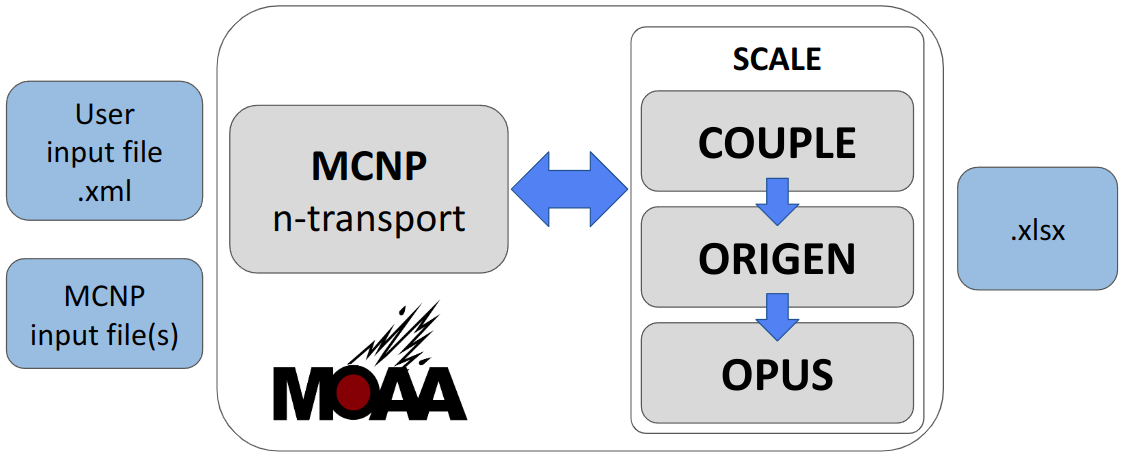
\includegraphics[width=0.90\linewidth]{figures/diagram_2}
  \end{center}
  \caption{Graphical representation of MOAA's workflow.}
  \label{fig:workflow_1}
\end{figure}

% Figure \ref{fig:workflow_1} displays MOAA's main calculation workflow.
% %% UIF
% The creation of a MOAA application starts with the definition of a \gls{UIF} in \textit{.xml} format.
% The \gls{UIF} contains a set of required and optional settings for MOAA.
% The required settings are a list of irradiation cases, a list of decay times, and a list of MCNP cells defining the regions of interest.
% The irradiation case geometry and material definition are specified by the MCNP input file(s).

% %% MCNP
% MCNP is a general-purpose, continuous-energy, generalized-geometry, Monte Carlo radiation-transport tool that can track neutrons, photons, electrons, and other particles.
% The main advantage of the Monte Carlo method is its capability in modeling geometry and interaction physics without significant approximations.
% MOAA relies on MCNP for obtaining the geometry- and material-dependent parameters of the user-defined system - i.e., fluxes and one-group cross-sections - during the irradiation steps.

% % CHANGES IN MCNP INPUT
% To accommodate the MOAA calculations, the MCNP input files must undergo a few minimal modifications.
% First, the depleted cells sharing the same material definition require the duplication of the original material as each MOAA depleted cell requires an independent material definition.
% The reason for this is to accommodate the depletion of independent cells subject to individual flux levels, divergent depletion rates, and the resulting different material compositions.

% Second, while MOAA can handle the depletion of cells defined as repeated structures, it cannot handle the depletion when the same cell is present in different nested structures.
% For example, if cell 100 is nested in cells 300 and 900 (100$<$300$<$900), and cell 100 is also nested in cells 400 and 900 (100$<$400$<$900), MOAA can handle only one of the two nested structures in one given simulation.
% To handle both nested structures, cell 400 would have to be redefined as 300 if the geometry definition allows, and MOAA will be able to handle both occurrences simultaneously.

% Third, the volume of some depleted cells has to be calculated and specified within the MCNP input file.
% This is because MCNP can only calculate the volume of simple geometries, and the user must specify the cell volumes to avoid errors.
% For cells defined as repeated structures, the user must specify the volume of the whole material in those cells that is present in the geometry.
% Otherwise, MCNP will calculate the volume of only one cell.

% %% ORIGEN
% ORIGEN is a general-purpose point depletion and decay tool to calculate isotopic concentrations, radiation source terms, and decay heat.
%DIF <  ORIGEN is integrated into the SCALE Code System, which is a modeling and simulation suite for nuclear safety analysis and design.
%DIF >  ORIGEN is integrated into the SCALE code system, which is a modeling and simulation suite for nuclear safety analysis and design.
% MOAA uses the calculated parameters from the MCNP output files to define the SCALE input files.
% Besides ORIGEN, MOAA also uses the COUPLE and OPUS modules from SCALE.
% ORIGEN requires a single space and spectrum-weighted cross-section library that MOAA generates using COUPLE.
% Meanwhile, OPUS provides the ability to extract specific data from the ORIGEN output libraries, perform unit conversions, and generate data for post-calculation analysis.

% %% Output file
% Upon successful execution of a MOAA simulation, a number of files are created in the UIF directory based on the user-defined settings.
% The most common files are an execution log file \textit{MOAA.log} and a \textit{.xlsx} spreadsheet with the isotopic composition.
% The log file contains all the logging messages produced during the execution, which may include warnings and errors.
% The generated spreadsheets contain the isotopic composition at the end of the last irradiation step and after each decay step.
% % For further details on MOAA's workflow, refer to \cite{fairhurst_moaa_2022}.

Figure \ref{fig:workflow_1} displays MOAA's main calculation workflow.
The \gls*{UIF} defines a list of irradiation cases, a list of decay times, and a list of MCNP cells defining the regions of interest.
The irradiation case geometry and material definition are specified by the MCNP input file(s).

%% MCNP
MCNP is a general-purpose, continuous-energy, generalized-geometry, Monte Carlo radiation-transport tool that can track neutrons, photons, electrons, and other particles.
The main advantage of the Monte Carlo method is its capability to model geometry and interaction physics without significant approximations.
MOAA relies on MCNP for obtaining the geometry- and material-dependent parameters of the user-defined system - i.e., fluxes and one-group cross-sections - during the irradiation steps.

% CHANGES IN MCNP INPUT
To accommodate the MOAA calculations, the MCNP input files must undergo a few minimal modifications.
First, the independent depletion of cells sharing the same material composition requires an independent material definition in the input files.

Second, while MOAA can handle the depletion of cells defined as repeated structures, it cannot handle the depletion when the same cell is present in different nested structures.
For example, if cell 100 is nested in cells 300 and 900 (100$<$300$<$900), and cell 100 is also nested in cells 400 and 900 (100$<$400$<$900), MOAA can handle only one of the two nested structures in one given simulation.
To handle both nested structures, cell 400 would have to be redefined as 300 if the geometry definition allows, and MOAA will be able to handle both occurrences simultaneously.

Third, the volume of some depleted cells has to be calculated and specified within the MCNP input file.
For cells defined as repeated structures, the user must specify the volume of the whole material in those cells that is present in the geometry.

%% ORIGEN
ORIGEN is a general-purpose point depletion and decay tool to calculate isotopic concentrations, radiation source terms, and decay heat.
ORIGEN is integrated into the SCALE \DIFdelbegin \DIFdel{Code System}\DIFdelend \DIFaddbegin \DIFadd{code system}\DIFaddend , which is a modeling and simulation suite for nuclear safety analysis and design.
MOAA uses the calculated parameters from the MCNP output files to define the SCALE input files.
Besides ORIGEN, MOAA also uses the COUPLE and OPUS modules from SCALE.
ORIGEN requires a single space and spectrum-weighted cross-section library that MOAA generates using COUPLE.
Meanwhile, OPUS provides the ability to extract specific data from the ORIGEN output libraries, perform unit conversions, and generate data for post-calculation analysis.


\subsection{Delayed heating}

The delayed heating calculation can be separated into two parts.
The first part calculates the deposition of energy from charged particles \DIFdelbegin \DIFdel{$H_{ch}$}\DIFdelend \DIFaddbegin \DIFadd{$H_{\mathrm{ch}}$}\DIFaddend .
This part includes only the charged particles \DIFdelbegin \DIFdel{that originated }\DIFdelend \DIFaddbegin \DIFadd{originating }\DIFaddend in the geometry of the component of interest.
The second part calculates the deposition of energy from photons \DIFdelbegin \DIFdel{$H_{\gamma, Tr}$}\DIFdelend \DIFaddbegin \DIFadd{$H_{\mathrm{\gamma, Tr}}$}\DIFaddend .
Because photons deposit their energy globally, photon transport is required, and this includes the photons originating from across the reactor.

\DIFdelbegin \DIFdel{The }\DIFdelend \DIFaddbegin \DIFadd{Equation \ref{eq:heat} along with the }\DIFaddend following equations describe the delayed heating
\begin{align}
H\DIFdelbegin \DIFdel{_{T} }%DIFDELCMD < [%%%
\DIFdel{W}%DIFDELCMD < ] &%%%
\DIFdel{= H_{ch} + H_{\gamma, Tr}  }%DIFDELCMD < \label{eq-heat} \\
%DIFDELCMD < %%%
\DIFdel{H_{ch} }\DIFdelend \DIFaddbegin \DIFadd{_{\mathrm{ch}} }\DIFaddend [\DIFdelbegin \DIFdel{W}\DIFdelend \DIFaddbegin \DIFadd{\mathrm{W}}\DIFaddend ] &= H\DIFdelbegin \DIFdel{_{T, L} }\DIFdelend \DIFaddbegin \DIFadd{_{\mathrm{T,L}} }\DIFaddend - H\DIFdelbegin \DIFdel{_{\gamma, L} }\DIFdelend \DIFaddbegin \DIFadd{_{\mathrm{\gamma, L}} }\DIFaddend \\
H\DIFdelbegin \DIFdel{_{\gamma, Tr} }\DIFdelend \DIFaddbegin \DIFadd{_{\mathrm{\gamma, Tr}} }\DIFaddend [\DIFdelbegin \DIFdel{W}\DIFdelend \DIFaddbegin \DIFadd{\mathrm{W}}\DIFaddend ] &= 1.6022 \times 10^{-13} \DIFaddbegin \DIFadd{\mathrm{J} \cdot \mathrm{MeV}^{-1} }\DIFaddend \times \: ^* \! F8 [\DIFdelbegin \DIFdel{MeV}\DIFdelend \DIFaddbegin \DIFadd{\mathrm{MeV}}\DIFaddend ] \times \mathlarger{\sum}_i S_i \label{eq-ga-tr} \\
S\DIFdelbegin \DIFdel{_i[\gamma/s] }\DIFdelend \DIFaddbegin \DIFadd{_i[\mathrm{\gamma} \cdot \mathrm{s}^{-1}] }\DIFaddend &= \int_{E} \varphi^\gamma_i(E) dE \\
s_i [-] &= S_i / \mathlarger{\sum}_j S_j \label{eq-emiprob}
\end{align}
where \DIFdelbegin \DIFdel{$H_{T}$ }\DIFdelend \DIFaddbegin \DIFadd{$H_{\mathrm{T}}$ }\DIFaddend is the total heat deposited in the region of interest, \DIFdelbegin \DIFdel{$H_{ch}$ }\DIFdelend \DIFaddbegin \DIFadd{$H_{\mathrm{ch}}$ }\DIFaddend is the energy deposited in the region of interest by charged particles, \DIFdelbegin \DIFdel{$H_{\gamma, Tr}$ }\DIFdelend \DIFaddbegin \DIFadd{$H_{\mathrm{\gamma, Tr}}$ }\DIFaddend is the energy deposited in the region of interest resulting from the photon transport, \DIFdelbegin \DIFdel{$H_{T,L}$ }\DIFdelend \DIFaddbegin \DIFadd{$H_{\mathrm{T,L}}$ }\DIFaddend is the total decay heat, \DIFdelbegin \DIFdel{$H_{\gamma, L}$ }\DIFdelend \DIFaddbegin \DIFadd{$H_{\mathrm{\gamma, L}}$ }\DIFaddend is the total gamma heating, $^\ast F8$ is the energy deposition calculated by an $^\ast$F8 tally, $S_i$ is the total photon emission rate from the region $i$, $\varphi^\gamma_i(E)$ the photon source energy distribution from region $i$, and $s_i$ is the source cell emission probability.

Overall, the calculation scheme follows the formal 3-step process, in which MOAA conducts the first two steps, and multiple MCNP photon-transport simulations carry out the third step, calculating the delayed gamma heating.
As shown in Figure \ref{fig:workflow_2}, the nuclear heating calculation relies primarily on MOAA.
MOAA calculates \DIFdelbegin \DIFdel{$H_{T,L}$ and $H_{\gamma, L}$ }\DIFdelend \DIFaddbegin \DIFadd{$H_{\mathrm{T,L}}$ and $H_{\mathrm{\gamma, L}}$ }\DIFaddend in the component of interest assuming those to be locally deposited.

\begin{figure}[htbp!]
  \begin{center}
    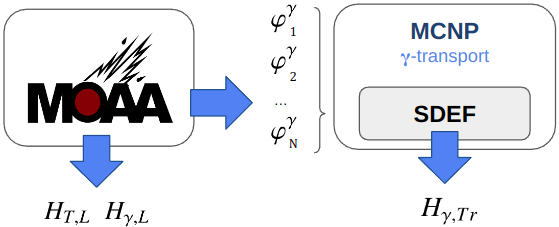
\includegraphics[width=0.90\linewidth]{figures/heat_flow}
  \end{center}
  \caption{Delayed heating calculation scheme relying on MOAA.}
  \label{fig:workflow_2}
\end{figure}

MOAA calculates $\varphi^\gamma_i(E)$ for all the cells defined by the user as contributors to the delayed heating.
The MCNP photon-transport simulations require the definition of a fixed source for these cells.
The source energy distribution is specified with $\varphi^\gamma_i(E)$.

The photon-transport calculation can be performed with multiple simulations, wherein one simulation obtains the heat contribution for one source cell, or with one simulation, wherein the simulation obtains the heat contribution for all the source cells simultaneously.
While the former allows the determination of individual contributions from the different cells, the latter is computationally less expensive.
Nonetheless, the latter requires the definition of the cell emission probabilities $s_i$ using equation \ref{eq-emiprob}.

The source spatial distribution is assumed uniform in each source cell.
For uniformly sampling the birth of a particle in a cell, MCNP uses the enclosing volume rejection method, which requires the user definition of a volume enveloping the source cell.
The randomly sampled points in the volume are accepted as source points only if they fall inside the source cell.
% In the calculation workflow described here, the user can define either a parallelepiped or a cylinder as the enclosing volume.
Finally, the photon transport estimates $^\ast F8$, which allows the calculation of \DIFdelbegin \DIFdel{$H_{\gamma, Tr}$ }\DIFdelend \DIFaddbegin \DIFadd{$H_{\mathrm{\gamma, Tr}}$ }\DIFaddend (eq. \ref{eq-ga-tr}).


\section{Results}
\label{sec:results}

This section presents and discusses the results of two applications.
The first application consists of the delayed heating calculation of an ATR experiment.
The second application analyzes the delayed heating in various structures in the RA-6 reactor.


\subsection{ATR experiment}

% ATR: Intro
The \gls*{ATR} is a 250-MWth high flux test reactor located at the Reactor Technology Complex of the \gls*{INL}.
The ATR was designed to provide an irradiation test environment for conducting a variety of experiments, to study the effects of radiation on reactor structural and fuel materials, and to produce medical and industrial isotopes \cite{ICSBEP, tomberlin_advanced_2002}.

% ATR: reactor description
The ATR core contains 40 fuel elements arranged in a serpentine annulus between and around nine flux traps, as shown in Figure \ref{fig:atr}.
Each fuel element consists of 19 parallel, curved, aluminum-clad fuel plates forming a 45-degree sector of a right circular cylinder.
The fuel arrangement gives the reactor core a clover-leaf configuration, which allows the \gls*{ATR} to be operated at different power levels in the \DIFdelbegin \DIFdel{corner lobes }\DIFdelend \DIFaddbegin \DIFadd{five lobes (NW, NE, C, SW, SE)}\DIFaddend , allowing for independent testing conditions within the same operating cycle.
Within each fuel plate, the fuel meat consists of highly enriched (93 wt\%) uranium aluminide (UAl$_x$) fuel powder dispersed in aluminum.
Plates 1 through 4 and 16 through 19 contain natural boron carbide (B$_4$C) powder as a burnable poison.

% ATR figure of the model
\begin{figure}[htbp!] %or H 
    \centering
    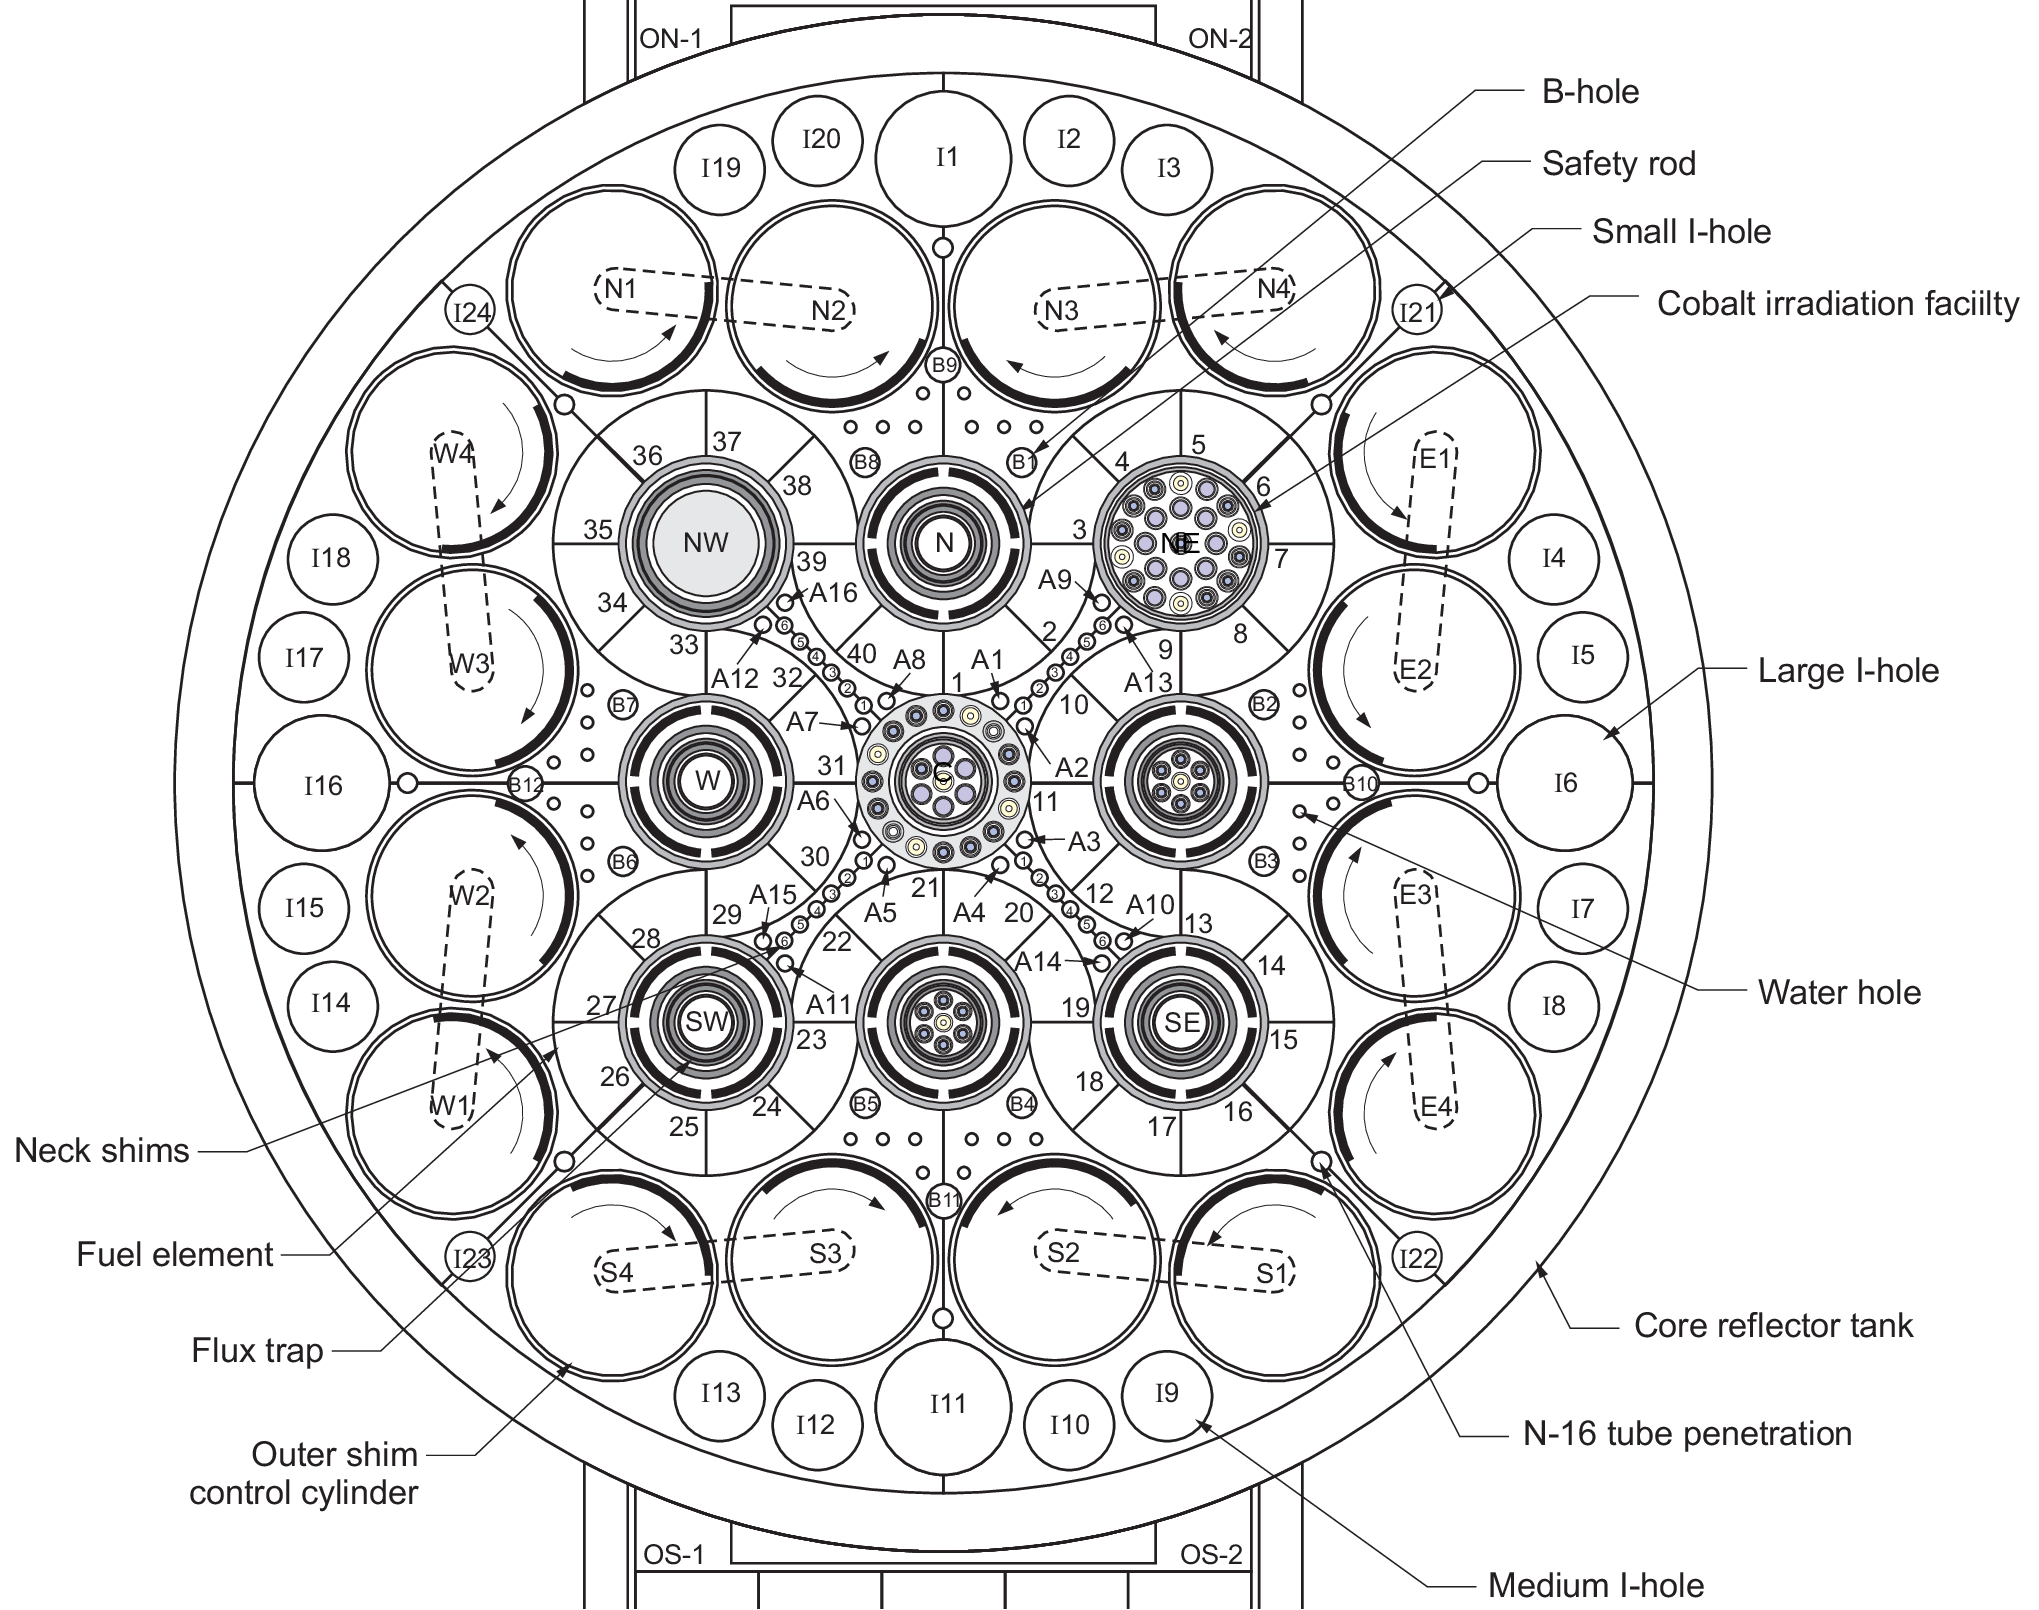
\includegraphics[width=0.90\linewidth]{figures/atr2}
    \hfill
    \caption{Top view of the ATR. Image reproduced from \cite{ICSBEP}.}
    \label{fig:atr}
\end{figure}

% Experiment positions
The reactor has 9 flux trap positions and 68 additional irradiation positions inside the reactor core reflector tank.
The center capsule facility is surrounded by the H-hole irradiation facility, which contains 10 cobalt baskets, 4 flux monitor holders, and 2 N-16 flow tubes.
The neck shim housing is the structural guide for the 24 neck shim and regulating rods, as well as 8 inner and 8 outer A-holes.
The beryllium reflector fills the space between the fuel annulus and the core reflector tank, and it hosts the outer shim control cylinders (OSCC), irradiation holes, and water holes.
The irradiation holes include a total of 8 small B-holes, 4 large B-holes, 4 small I-holes, 16 medium I-holes, 4 large I-holes, and 4 round and 4 square N-16 monitor holes.

% Describe model
This work uses an MCNP model representing the ATR critical experiment evaluation designated as Cycle 103A-2 that was performed in 1994.
This critical evaluation was part of a nuclear re-qualification program that followed the core internals change-out.
The critical configuration was defined by the following parameters: 40 fresh fuel elements, OSCC set to 51.8 degrees, 22 shim rods fully inserted, 2 regulating rods fully withdrawn, and 6 safety rods fully withdrawn.

The ATR critical evaluation was first published by the OECD NEA Nuclear Science Committee in the September 2005 Edition of the International Handbook of Evaluated Criticality Safety Benchmark Experiments (ICSBEP Handbook) \cite{ICSBEP}.
% ATR-FUND-RESR-001 was approved by the IRPhEP in October of 2008 and is published in the International Handbook of Evaluated Reactor Physics Benchmark Experiments under its ICSBEP Identifier, HEU-MET-THERM-022.
% % The report is published in the original ICSBEP format and contains only evaluation of the critical state measurement.
The original benchmark model uses the evaluated continuous energy ENDF/B-V cross-section data for 27 $^{\circ}$C.
% TODO/MAYBE: make sure that I am using this cross-section library
This work uses the ENDF/B-VIII.0 cross-section library for the isotopes included in it.
The remaining isotopes use the cross-section data of the original model.
% The benchmark model 
The model uses 10$^4$ histories per generation with 250 and 3750 inactive and active cycles.
This work considers the reactor composition at the \gls*{BOC} based on the available ATR model.

% Problem definition
This demonstration exercise focuses on the delayed heating of the A1 experiment position.
The A1 experiment position is an inner A-hole, and it is hosted by the neck shim housing.
\DIFdelbegin \DIFdel{The diameter of the hole is 0.625 in.
}\DIFdelend This exercise considers an experiment sample \DIFaddbegin \DIFadd{of 1.46 cm in diameter and 168.27 cm in height }\DIFaddend made of aluminum.

% POWER
Although the ATR maximum power rating is 250 MWth, most contemporary experiments do not require such a level, and the reactor operates at a much lower power.
This work considers for the calculations a total operating power of 110 MWth that is equally distributed among the \DIFdelbegin \DIFdel{5 }\DIFdelend \DIFaddbegin \DIFadd{five }\DIFaddend lobes.
% Irradiation time
The irradiation time is 30 days, and the decay is recorded in seven non-uniformly distributed steps up to 12 hours after shutdown.

% Contributing cells
As the experiment position is in the core region between the fuel assemblies, the calculations assume that the fission products generate a much higher gamma source intensity than the activation products in the neighboring cells.
Hence, the contribution of the reactor components surrounding the experiment is neglected.
The only considered contributors to the heating are all the fuel plates and the experiment itself.


% ATR results
\subsection{ATR results}

% CHANGES IN MCNP INPUT
To accommodate the MOAA calculations, the MCNP input file underwent the following modifications.
The ATR model defines 19 different material compositions that all fuel elements share for their 19 different fuel plates.
The material definitions of each fuel plate were duplicated for each fuel element to allow for their independent definition.
Additionally, the volume of each fuel plate was calculated and added into the MCNP input file.

Figure \ref{fig:atr-time} presents the experiment heat production over time.
\DIFdelbegin \DIFdel{$H_{\gamma,Tr}$ }\DIFdelend \DIFaddbegin \DIFadd{$H_{\mathrm{\gamma, Tr}}$ }\DIFaddend was calculated for 41 independent photon-transport simulations, wherein each simulation accounts for the contribution to delayed gamma heating of each fuel assembly and the experiment itself.

The gamma heating immediately after shutdown is 849.2 W, and the heating due to charged particles is 56.32 W, which equals to 6.6\% of the total heating in the experiment.
The self-gamma heating is 5.8 W, which is equal to 0.73\% of the total delayed gamma contribution and 0.68\% of the total heating.
These results show that the self heating in aluminum is very low and validate the initial simplification of neglecting the surrounding structure contributions given that both the experiment and the structures are made of aluminum.

Additionally, the heating due to charged particles decays much faster than the gamma heating and becomes negligible one hour after shutdown.
The gamma heating decays to 100 W at approximately six hours after shutdown.

\begin{figure}[htbp!] %or H 
    \centering
    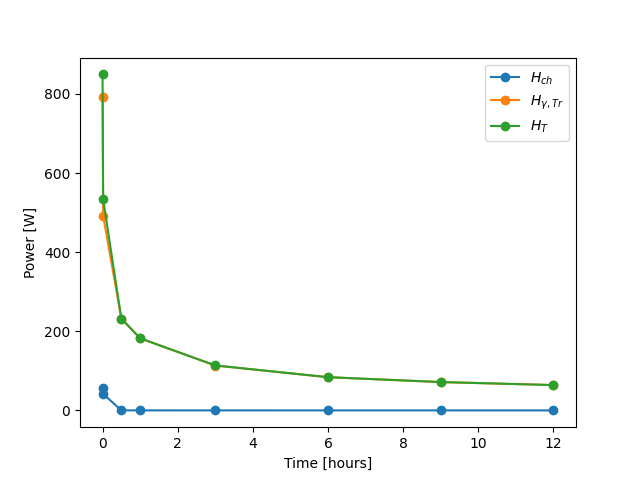
\includegraphics[width=0.90\linewidth]{figures/atr_decay_heat_time}
    \hfill
    \caption{Shutdown heating rate over time in the ATR A1 experiment position for an aluminum sample.}
    \label{fig:atr-time}
\end{figure}

Figure \ref{fig:atr-contrib} shows the contribution to the total heat in percentage by each fuel assembly and the experiment immediately after shutdown.
The largest contributions to the heating in the sample come from the fuel assemblies 1, 10, 40, 2, 11, 9 with contributions of more than 3\%.
These assemblies are the closest in distance to the experiment position.
Additionally, the sample produced a self-heating of 7.3\%, from which 6.6\% came from the charged particles and 0.7\% from the gamma particles.
% This confirms the assumption that the gamma heating from the fission products is considerably larger than the gamma heating from activation products in the vicinity of the fuel assemblies.

% Maybe talk about the following:
% The neck shim housing has an elongated shape.
%DIF <  So, several of the gammas originated here will not be deposited in the experiment position but in the fuel elements.
%DIF <  Additionally, our method considers that the gamma are originated uniformly across the cell geometry.
%DIF >  So, several of the gammas originating here will not be deposited in the experiment position but in the fuel elements.
%DIF >  Additionally, our method considers that the gamma originate uniformly across the cell geometry.
% Which in this case a mesh based approach may be more accurate.

\begin{figure}[htbp!] %or H 
    \centering
    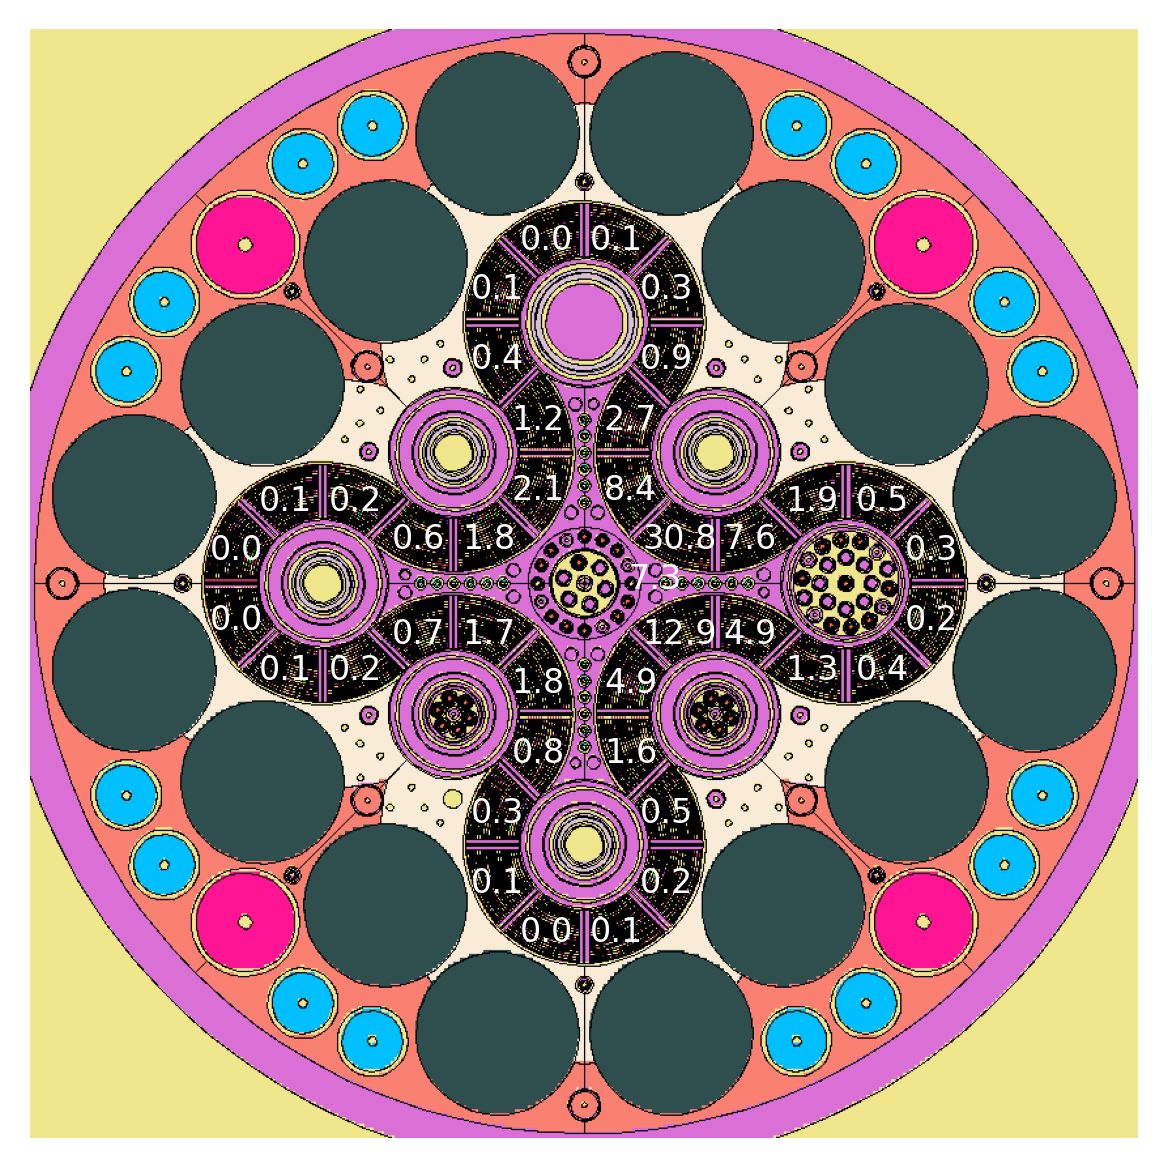
\includegraphics[width=0.90\linewidth]{figures/atr_contributions}
    \hfill
    \caption{Contribution by each source to the A1 experiment heat rate immediately after reactor shutdown, with the values expressed in (\%). The Figure is based on the MCNP model geometry, which is rotated 45$^{\circ}$ clockwise with respect to Figure \ref{fig:atr}.}
    \label{fig:atr-contrib}
\end{figure}


\subsection{RA-6 structures}

% Intro
The RA-6 is a 3-MWth open pool research reactor located at the Bariloche Atomic Center (CAB), a research and development center of the Argentine National Atomic Energy Commission (CNEA) \cite{ICSBEP}.
It was originally conceived as a teaching tool to support student training at the Balseiro Institute before its uses became diversified.
Current applications include neutron activation analysis, neutron radiography, and \gls*{BNCT}, among others.

% The reactor
The reactor core is composed of a fuel element arrangement, as shown in Figure \ref{fig:ra6-1}, that rests on a support grid inside a 2.4-m-diameter, 10.4-m-high stainless steel tank.
The tank is filled with demineralized light water, which acts as a coolant, moderator, and reflector.
The fuel elements are Material Test Reactor (MTR) type, composed of rectangular fuel plates with aluminum side plates.
The fuel meat consists of 19.7\% enriched uranium silicide (U$_3$Si$_2$) dispersed in an aluminum matrix.
There are two types of fuel elements: \DIFdelbegin \DIFdel{Normal Fuel Elements }\DIFdelend \DIFaddbegin \DIFadd{normal fuel elements }\DIFaddend (NFEs) and \DIFdelbegin \DIFdel{Control Fuel Elements }\DIFdelend \DIFaddbegin \DIFadd{control fuel elements }\DIFaddend (CFEs).
While an NFE is composed of 17 internal and two external fuel plates, a CFE is composed of 14 internal and 4 control guide plates.

% Support grid
The bottom plane of the core assembly rests 8.9-meters-deep on the support grid, which is a 20 cm-thick slab of 99.5\% pure aluminum.
Primary and secondary cylindrical holes allow the cooling of the internal and external fuel plates, respectively.
The primary holes have a diameter of 6.179 cm and are arranged in a rectangular \DIFdelbegin \DIFdel{8x10 }\DIFdelend \DIFaddbegin \DIFadd{8 x 10 }\DIFaddend array with 7.7-cm pitch in the x-direction and 8.1-cm pitch in the y-direction.
The secondary holes have a diameter of 2.225 cm and are centered between the primary holes.

% BNCT filter
On a side of the fuel element arrangement, there is a neutron filter that works as a source for \gls*{BNCT}, as shown in Figure \ref{fig:ra6-2}.
The neutron filter for the \gls*{BNCT} facility is an 87.6-cm-long, 77.1-cm-wide, 82.35-cm-high \DIFdelbegin \DIFdel{aluminum }\DIFdelend container.
The filter is filled along the 87.6-cm dimension with the following materials: 17 cm of aluminum bricks, a 0.15-cm-thick cadmium sheet, 10 cm of aluminum, a 0.15-cm-thick cadmium sheet, and the rest is filled with alumina \DIFaddbegin \DIFadd{(Al$_2$O$_3$) }\DIFaddend bricks.

\begin{figure}[htbp!] %or H 
    \centering
    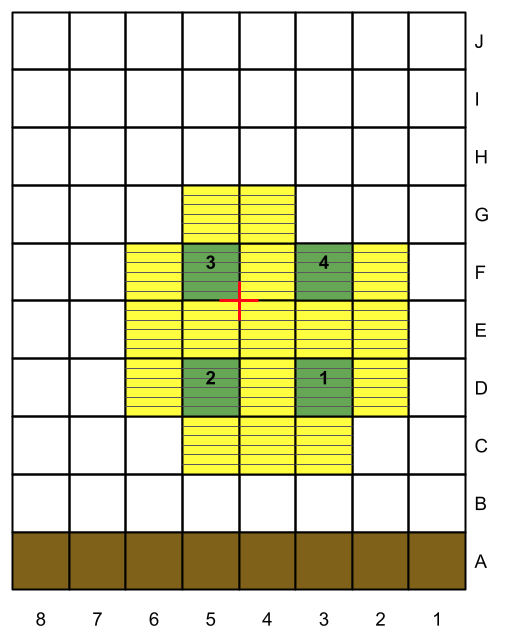
\includegraphics[width=0.55\linewidth]{figures/ra6_core2}
    \hfill
    \caption{Top view of the RA-6 critical configuration. NFEs in yellow, CFEs in green, and BNCT filter in brown. Red cross denotes the center of the reactor pool. Image reproduced from \cite{ICSBEP}.}
    \label{fig:ra6-1}
\end{figure}

\begin{figure}[htbp!] %or H 
    \centering
    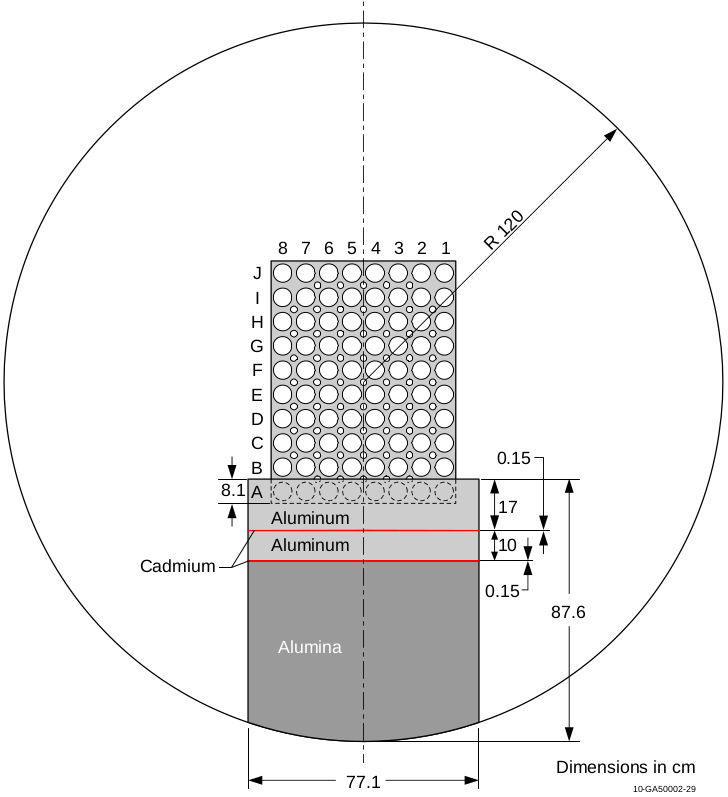
\includegraphics[width=0.70\linewidth]{figures/bnct}
    \hfill
    \caption{Top view of the RA-6 support grid and BNCT filter. Image reproduced from \cite{ICSBEP}.}
    \label{fig:ra6-2}
\end{figure}

% The model
The RA-6 reactor operated for 20 years with spent \gls*{HEU} fuel from a higher power reactor and was reconverted to \gls*{LEU} fuel in 2008.
The RA-6 critical experiment reported in this evaluation corresponds to the 2008 configuration utilized in the startup program.
% RA6-FUND-RESR-001 
This critical evaluation was first published by the OECD NEA Nuclear Science Committee in the September 2010 Edition of the ICSBEP Handbook.
% RA6-FUND-RESR-001 was first published by the IRPhEP in the March 2013 Edition of the International Handbook of Evaluated Reactor Physics Benchmark Experiments under its ICSBEP Indentifier, IEU-COMP-THERM-014.
% The report contains only an evaluation of the critical state measurement.
This work considers the reactor composition at the \gls*{BOC} based on the available RA-6 model and uses the evaluated continuous energy ENDF66 cross-section data for 27 $^{\circ}$C, which is defined in the original benchmark model.
% % TODO/MAYBE: make sure that I am using this cross-section library
% This work uses the ENDF/B-VII.1 cross-section library for the isotopes included in it.
% The remaining isotopes use the original model cross-section data.
% The benchmark model 
The simulation uses 10$^4$ histories per generation with 50 and 4000 inactive and active cycles.

% The calculations
Although not shown in the MCNP model, the reactor core has several surrounding components, such as primary pipes, the stainless steel tank, and neutron beam extraction tubes.
The analysis of delayed heating in these components could be worthwhile but were omitted as the MCNP model excluded them.
Hence, this work calculates the delayed heating on the most important structural components in the model, i.e., the support grid and the BNCT filter.

% POWER
The RA-6 was originally designed to operate at 1 MWth and the 2008 startup program included a reactor power upgrade to 3 MWth.
Although the RA-6 maximum power rating is 3 MWth, it normally operates at a lower power.
This work considers operating powers of 1 and 3 MWth and compared their respective results.
% Irradiation time
In this work, the \DIFdelbegin \DIFdel{rector }\DIFdelend \DIFaddbegin \DIFadd{reactor }\DIFaddend operated for 1 year and the depletion was calculated in four 3-month steps.
% Contributing cells
The considered contributors to the heating are the fuel plates, the support grid, and the BNCT filter.


\subsection{RA-6 results}

% CHANGES IN MCNP INPUT
To accommodate the MOAA calculations, the MCNP input file underwent the following modifications.
First, even though the RA-6 model distinguishes between five different types of fuel plates: internal plates in the NFEs, internal plates with burnable poisons in the NFEs, external plates in the NFEs, fuel plate with burnable poisons in the CFEs, and fuel plate without burnable poisons in the CFEs, the original MCNP input file defines all of them with the same material definition.
Additionally, several layers of the BNCT filter and the support grid are made of pure aluminum, and the original MCNP input file defines the aluminum only once.
Finally, the BNCT filter uses two cadmium layers that share the same material definition in the original MCNP input file.
All material definitions of these components were duplicated to allow for their independent definition.
Second, the original MCNP input file defines the four CFEs using nested structures with independent cells, but as their definition is identical, a minimal universe renumbering allowed their simultaneous modeling in MOAA.
Third, the volume of each fuel plate type, the volume of the different BNCT filter layers, and the volume of the support grid were calculated and added into the MCNP input file.

Figure \ref{fig:ra6-3} displays the delayed heating in the support grid and the different BNCT filter layers for operating powers of 1 and 3 MWth, and Table \ref{tab:ra6-res} shows the density of deposited heat in the different structures.
The highest deposited heat occurs in the first BNCT layer, while the highest density of deposited heat occurs in the second BNCT layer, which is the first cadmium layer in the filter.
For the first, third, and fifth layers of the BNCT filter, the density of deposited heat decreases due to an increase in the spatial distance from the core.
However, the fifth layer has a larger deposited heat than the third layer due to its considerably larger volume.
The deposited heat in the cadmium sheets is considerably smaller than for the rest of the BNCT layers due to their smaller volume.
Table \ref{tab:ra6-res} also shows the comparison between the results for 1 and 3 MWth.
A three times fold increase in operation power is translated into an increase in delayed heating of between 2.60 to 2.90 in the reactor structures.

\begin{figure}[htbp!] %or H 
    \centering
    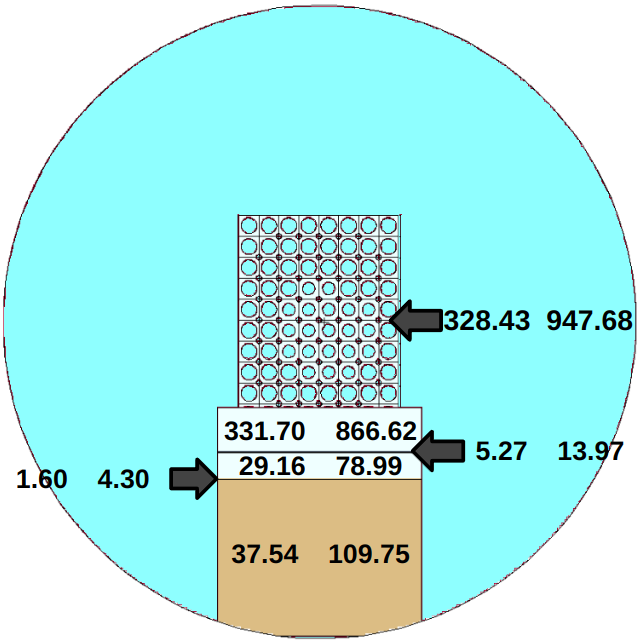
\includegraphics[width=0.80\linewidth]{figures/results_b}
    \hfill
    \caption{Delayed heating in the RA-6 reactor structures. Values expressed in \DIFdelbeginFL \DIFdelFL{$W$}\DIFdelendFL \DIFaddbeginFL \DIFaddFL{W}\DIFaddendFL . Left: values corresponding to 1 MWth. Right: values corresponding to 3 MWth.}
    \label{fig:ra6-3}
\end{figure}

\begin{table}[htbp!]
  \centering
  \caption{Main results for delayed heating in the RA-6 reactor structures for an operating power of 1 MWth. \DIFdelbeginFL \DIFdelFL{Values expressed in $W$}\DIFdelendFL \DIFaddbeginFL \DIFaddFL{$V$ is the cell volume}\DIFaddendFL .}
  \label{tab:ra6-res}
  \begin{tabular}{cccc}
    \toprule
                    \DIFdelbeginFL %DIFDELCMD < 

%DIFDELCMD <                     %%%
\DIFdelendFL & \DIFdelbeginFL \DIFdelFL{$H_{T, 1MW}/V [W/m^3]$  }\DIFdelendFL \DIFaddbeginFL \DIFaddFL{$H_{\mathrm{T, 1MW}}/V$ }[\DIFaddFL{W $\cdot$ m$^{-3}$}]  \DIFaddendFL & \DIFdelbeginFL \DIFdelFL{$H_{T, 3MW}/V [W/m^3]$  }\DIFdelendFL \DIFaddbeginFL \DIFaddFL{$H_{\mathrm{T, 3MW}}/V$ }[\DIFaddFL{W $\cdot$ m$^{-3}$}]  \DIFaddendFL & \DIFdelbeginFL \DIFdelFL{$ \frac{H_{T, 3MW}}{H_{T, 1MW}} $  }\DIFdelendFL \DIFaddbeginFL \DIFaddFL{$\frac{ H_{\mathrm{T, 3MW}} }{ H_{\mathrm{T, 1MW}} }$  }\DIFaddendFL \\
    \midrule
    Support grid    &  3291.14                &  9496.55                &  2.89    \\
    BNCT 1st layer  &  3073.12                &  8029.02                &  2.61    \\
    BNCT 2nd layer  &  5533.52                & 14668.54                &  2.65    \\
    BNCT 3rd layer  &   459.27                &  1244.10                &  2.71    \\
    BNCT 4th layer  &  1680.01                &  4515.01                &  2.69    \\
    BNCT 5th layer  &   102.13                &  298.57                 &  2.92    \\
    \bottomrule
  \end{tabular}
\end{table}


\section{Conclusion}
\label{sec:conclusion}

% Intro
Safety analyses in research reactors require the estimation of heat deposited in experiments and reactor structures after reactor shutdown.
These analyses establish the heat-source term of those components, and the subsequent thermal-hydraulics calculations determine if an accident could jeopardize their integrity.
Additionally, detailed calculations help guide the optimization process of the design of irradiation targets.

In general, existing research reactor safety analyses have a strong focus on the reactor core and assume that the energy released after shutdown is deposited locally in the region of interest.
Moreover, many software packages rely on the same assumption, which may be inadequate in some cases.
On the other hand, an accurate assessment of the deposited energy across the reactor geometry allows for better determination of the heat removal requirements and ensures an effective cool down.
Instead of assuming locally deposited heat, this work utilized detailed methods to target the specific reactor regions.

% Background
This article discusses various delayed heating calculation methods, and several publications relying on them.
The methods can be summarized into three main approaches: the formal 3-step process, the PIKMT method, and the D1S method.
Overall, the discussion gave rise to the choice of an approach for the calculation workflow used in this work.
The fact that the formal 3-step process accounts for the activation product decay and the time evolution after shutdown gives the method prevalent attributes over the PIKMT and D1S methods.
Therefore, this work introduced a delayed heating calculation workflow based on the formal 3-step process that relies on MOAA.

% Method
MOAA is a python package that couples MCNP and ORIGEN to streamline the calculation of the experiment source terms for the \gls*{ATR} and the \gls*{TREAT}.
This article briefly discussed the MOAA workflow, with the main focus on the delayed heating calculation workflow.
The delayed heating calculation relies on MOAA for conducting the first two steps of the process, while the third step is conducted by multiple MCNP photon transport simulations.

% Results
Finally, this article demonstrated the delayed heating calculation capabilities by presenting two nuclear engineering exercises.
These exercises include the delayed heating in an ATR experiment and the RA-6 structures.
For the ATR experiment, the results showed the time evolution of the delayed heating up to 12 hours after shutdown as well as the contribution to the heating from the different sources in the reactor.
For the RA-6 structures, the results displayed the delayed heating in several of the structural components and the comparison of the heating values for different power levels.

% Conclusions
As discussed in the results section, the calculation workflow can accommodate almost any MCNP input file, with some minimal modifications.
Overall, this article presented delayed heating capabilities that rely on MOAA and that can be applied to any reactor.


\pagebreak

\section*{Acknowledgments}

This research made use of the resources of the High Performance Computing Center at the \gls*{INL}, which is supported by the Office of Nuclear Energy of the U.S. Department of Energy and the Nuclear Science User Facilities under Contract No. DE-AC07-05ID14517.

\pagebreak

\bibliographystyle{style/ans_js}  % custom ANS journal submission template bibliography style
\DIFdelbegin %DIFDELCMD < \bibliography{bibliography}
%DIFDELCMD < %%%
\DIFdelend \DIFaddbegin \bibliography{revised_bibliography}
\DIFaddend 

\end{document}
